\chapter{Introdução}

\begin{figure}[htbp]
  \centering
  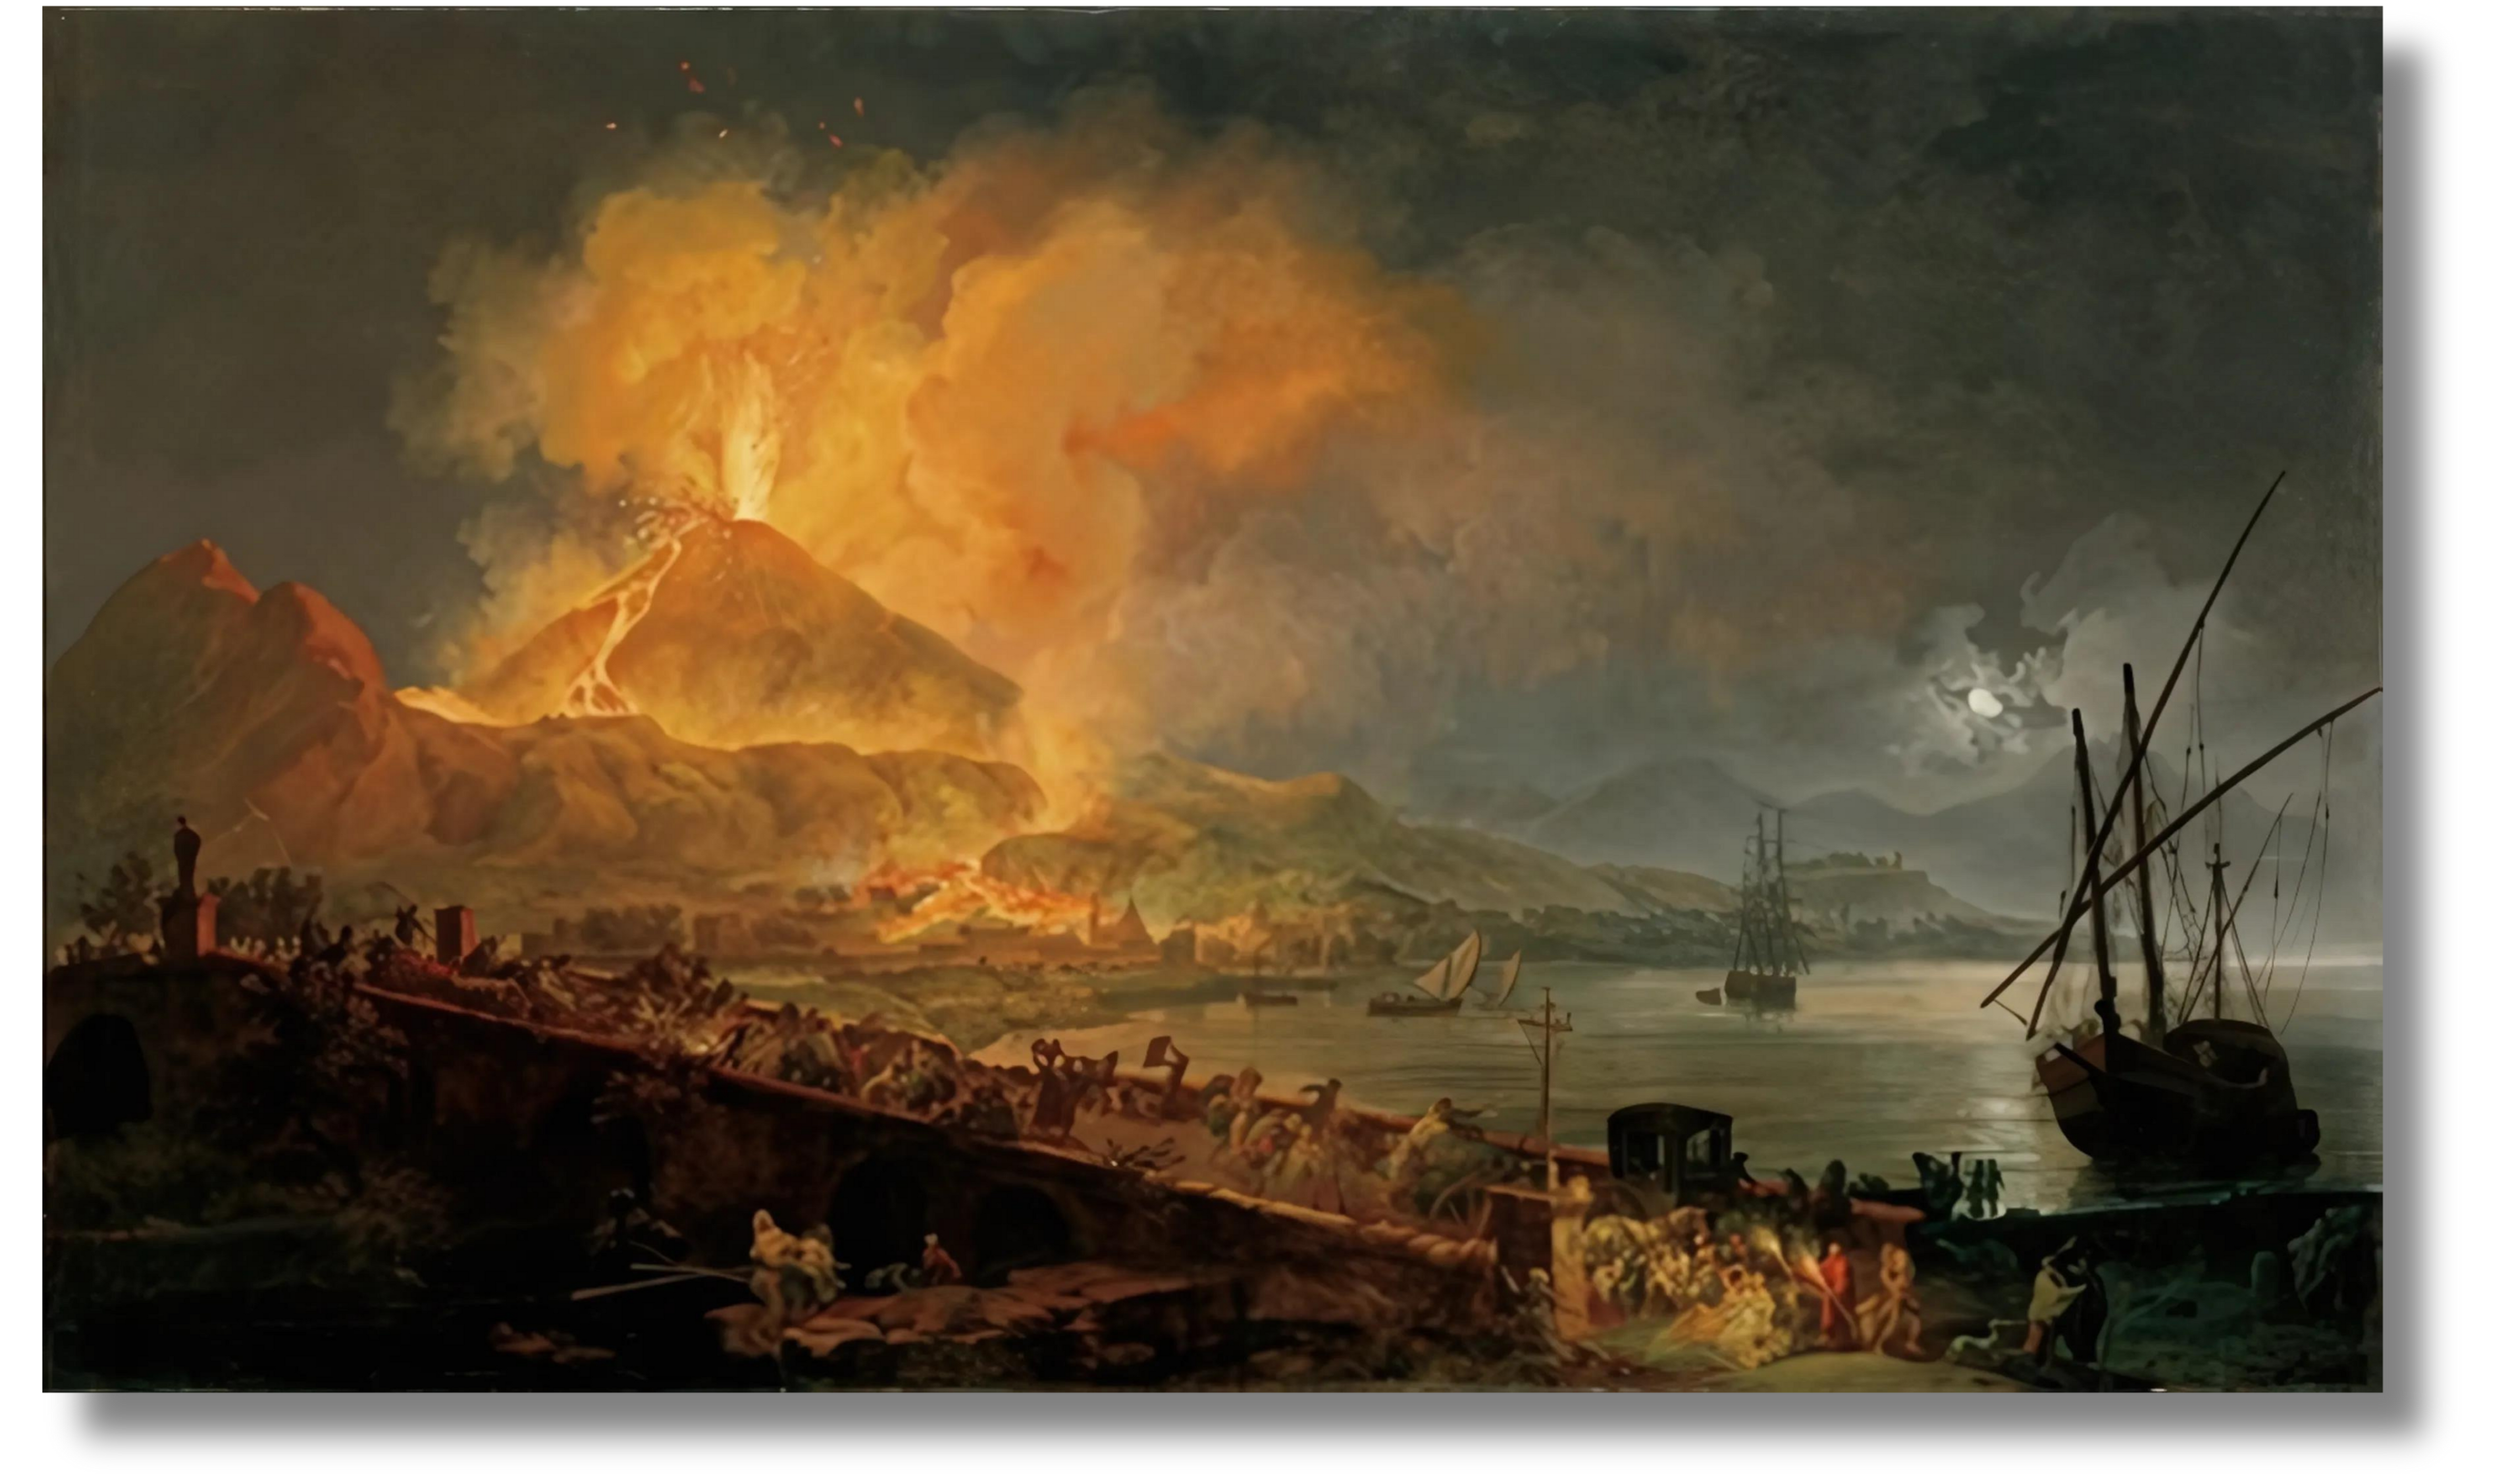
\includegraphics[width=0.9\textwidth]{The Eruption of Mt. Vesuvius.png}
  \caption{\fontsize{8}{8}\selectfont Fazer}
  \label{fig:exemplo}
\end{figure}

\fontsize{12}{14}\selectfont
O período iluminista expôs ainda mais a busca incessante da sociedade pelo conhecimento e constante busca por respostas novas para conceitos antigos, de modo a fascinar cada vez mais os seres acerca dos mistérios e indagações referentes ao “natural”. Tal incessante busca e embelezamento de uma reinterpretação humana sobre a natureza influenciou na visão – de certa forma – admiradora dos humanos por fenômenos naturais notáveis como os vulcões, expondo a dualidade do terror e deslumbramento no que diz respeito, principalmente, à erupção. Tal processo foi vítima de debates, imaginações e embelezamento artístico pelos filósofos, artistas e cientistas da época, sendo visto como uma manifestação visceral que indicava o poder e transformação da dita “Mãe-Natureza”.

Tal fascínio pelo poder e imponência de um vulcão e o fogo que advinha dele gerou o desejo de manipulação do próprio fogo pelos humanos, de maneira que o brilho das labaredas visto na lava se tornou objeto de estudo e desejo até o controle dele por meio dos fogos de artifício, que seguiu os princípios da cultura popular da época. Tais objetos eram muito mais do que somente brilhos no céu e festejos, era a certeza de que a ciência poderia levar o mundo humano a lugares e poderes inimagináveis de dominar – pelo menos simbolicamente – a potência da natureza, gerando uma bela e cintilante homenagem ao progresso.